\subsection{Insertion Sort}

\subsubsection{Core Concepts}
Insertion sort orders a list of values by repetitively inserting a particular value into a sorted subset of the list. More specifically, consider the first item to be a sorted sublist of length 1, insert second item into sorted sublist, shifting first item if needed. Insert third item into sorted sublist, shifting items 1-2 as needed. Repeat until all values have been inserted into proper positions. ~\cite{ref1}

\vspace{5pt}

\subsubsection{Step-by-step Explaination}
\begin{itemize}[label=-]
    \item Step 1: Assume the first element is already sorted. Pick the next element and find its correct position among the already sorted elements.
    \item Step 2: Shift all the elements greater than the picked element to one position ahead to make space for the picked element.
    \item Step 3: Insert the picked element into its correct position.
    \item Step 4: Repeat the above steps for all elements in the array.
\end{itemize}

\subsubsection{Complexity Analysis:}
At each iteration, the array is divided into two subarrays, the left part is sorted, and the right part is unsorted. Accelerate the search using binary search.

\textbf{Iteration 1:} Perform 1 comparison to find the insertion position for $a[1]$

\textbf{Iteration 2:} Perform at least 1 comparison, at most 2 comparisons to find the insertion position for $a[2]$

...

\textbf{Iteration $n - 1$:} Perform at least 1 comparison, at most $(n - 1)$ comparisons to find the insertion position for $a[n - 1]$, ending the algorithm

In each iteration, the number of assignments is equal to the number of comparisons made.

Let $f(n)$ be the cost function of the algorithm (based on the number of comparisons and assignments):

\[
f(n) = (n_1 + n_2 + \ldots + n_{n-1}) \times 2 \quad \text{where:} \quad n_1 = 1, \quad n_2 \in [1, 2], \quad n_3 \in [1, 3], \ldots, \quad n_{n-1} \in [1, n - 1]
\]

\textbf{Time Complexity:}
\begin{itemize}
    \item Best-case: $O(n)$
    \item Average-case: $O(n^2)$
    \item Worst-case: $O(n^2)$
\end{itemize}
\textbf{Space complexity:} O(1) (in-placed)

\vspace{5pt}

\textbf{An example of Insertion sort} ~\cite{ref1}

\begin{figure}[h]
    \centering
    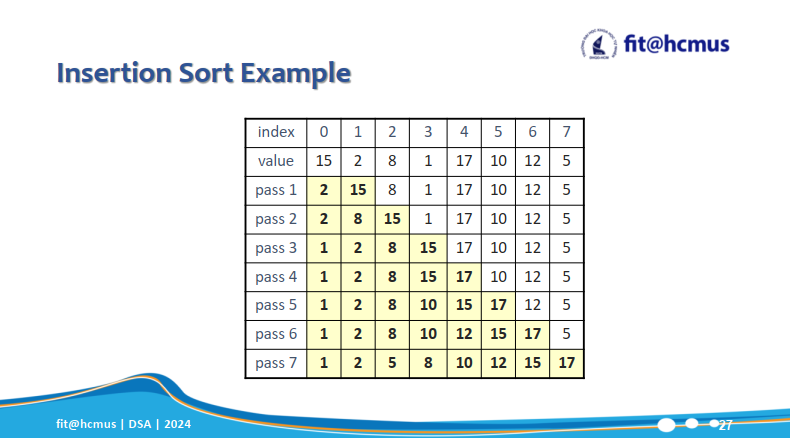
\includegraphics[scale=.40]{Figures/sort_demo/insertion.png}
    \caption{Insertion Sort Demo}
    \label{fig:enter-label}
\end{figure}